
% header %{{{1

\documentclass[tikz, border=1mm]{standalone}

\usepackage{amsmath}

\usetikzlibrary{calc,angles,quotes,shapes.geometric}

% document %{{{1

% opening %{{{2

\begin{document}
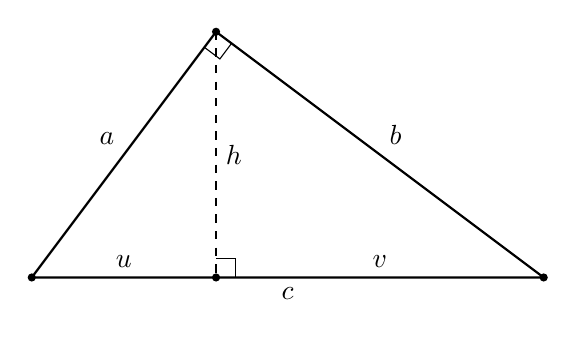
\begin{tikzpicture}[scale=1.3]

% parameters %{{{2

	% ---- triangle 3 - 4 - 5
	% ---- arctan(4/3) in degrees

	\def\ang{53.13}

% coordinates %{{{2

	\coordinate (A) at (0,0);
	\coordinate (B) at ({3*cos(\ang)},{3*sin(\ang)});
	\coordinate (C) at (5,0);

	% ---- feet of altitude from B to AC

	\coordinate (D) at ({3*cos(\ang)},0);

% triangle %{{{2

	\draw[thick] (A) -- (B) -- (C) -- cycle;

	% ---- altitude

	\draw[dashed] (B) -- (D);

% vertices, points, dots %{{{2

	\fill (A) circle (0.4mm);
	\fill (B) circle (0.4mm);
	\fill (C) circle (0.4mm);
	\fill (D) circle (0.4mm);

% sides labels %{{{2

	\node[above left]  at ($(A)!0.5!(B)$) {$a$};
	\node[above right] at ($(B)!0.5!(C)$) {$b$};
	\node[below] at ($(A)!0.5!(C)$) {$c$};

	% ---- segment labels on altitude projection

	\node[above] at ($(A)!0.5!(D)$) {$u$};
	\node[above] at ($(D)!0.5!(C)$) {$v$};

% right angles markers %{{{2

	\pic [draw, angle radius=7pt, angle eccentricity=1]
	{right angle = A--B--C};
	\pic [draw, angle radius=7pt, angle eccentricity=1]
	{right angle = B--D--C};

	% ---- height label

	\node[right] at ($(B)!0.5!(D)$) {$h$};

% closing %{{{2

\end{tikzpicture}
\end{document}
